% Chương 3: Phương pháp và kiến trúc hệ thống

\chapter{Phương pháp và kiến trúc hệ thống}

\label{Chapter3}

%----------------------------------------------------------------------------------------

\section{Tổng quan kiến trúc hệ thống}

\begin{figure}[h!]
    \centering
    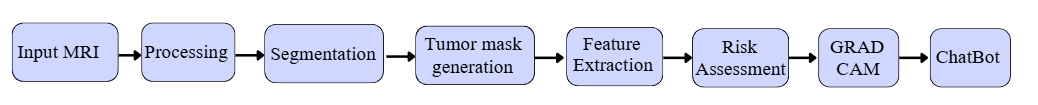
\includegraphics[width=1\textwidth]{Figures/Chapter/Chapter5.png}
    \caption{Pineline phương pháp.}
    \label{fig:pineline}
\end{figure}

%----------------------------------------------------------------------------------------
\subsection*{I. Giai đoạn 1 -- Tiếp nhận và xác thực yêu cầu}
%----------------------------------------------------------------------------------------

\subsection*{1. Endpoint REST}

Endpoint duy nhất cho dự đoán là \texttt{POST /api/v1/predict}, định nghĩa trong \texttt{app/api/predict.py}. FastAPI nhận file qua \texttt{multipart/form-data} nhờ khai báo \texttt{UploadFile = File(...)}.

\subsection*{2. Input MRI}

Trước khi dữ liệu được đưa vào pipeline xử lý chính, hệ thống tiến hành một chuỗi kiểm tra nhằm đảm bảo tính hợp lệ và an toàn của tệp đầu vào. Các bước kiểm tra được thực hiện theo thứ tự như sau:

\begin{sloppypar}
\begin{enumerate}
    \item \textbf{Kiểm tra loại MIME}: Hệ thống xác minh trường \texttt{file.content\_type} phải thuộc nhóm \texttt{"image/"}. Nếu điều kiện không được thỏa mãn, yêu cầu sẽ bị từ chối với mã lỗi HTTP 400.

    \item \textbf{Kiểm tra dung lượng tệp}: Toàn bộ dữ liệu được đọc vào bộ nhớ thông qua lệnh \texttt{raw = await file.read()}. Nếu kích thước vượt quá ngưỡng 20\,MB (\texttt{len(raw) > 20\,MB}), hệ thống trả về mã lỗi HTTP 413 để hạn chế tải tài nguyên.

    \item \textbf{Kiểm tra tính toàn vẹn của ảnh}: Thư viện Pillow được sử dụng để thử mở dữ liệu ảnh. Trong trường hợp tệp bị hỏng hoặc không đúng định dạng, một ngoại lệ sẽ được kích hoạt và hệ thống phản hồi mã lỗi HTTP 422.
\end{enumerate}
\end{sloppypar}
%----------------------------------------------------------------------------------------
\subsection*{II. Giai đoạn 2 -- Tiền xử lý ảnh}
%----------------------------------------------------------------------------------------

\subsection*{1. Chuỗi biến đổi}

Module \texttt{utils/image\_utils.py} thực hiện một chuỗi bốn bước xử lý tuần tự nhằm biến đổi ảnh thô thành định dạng đầu vào phù hợp cho mô hình học sâu.

\begin{sloppypar}
\begin{enumerate}
    \item \textbf{Giải mã và chuẩn hóa không gian màu}: Dữ liệu ảnh được đọc từ byte stream thông qua \texttt{Image.open(BytesIO(raw))} của Pillow. Sau đó, ảnh được chuyển về định dạng RGB để đảm bảo tính nhất quán giữa các trường hợp ảnh đầu vào như grayscale, RGB hoặc RGBA, tất cả đều được đưa về ba kênh màu chuẩn.

    \item \textbf{Thay đổi kích thước ảnh}: Ảnh được resize về kích thước cố định $256 \times 256$ bằng phương pháp nội suy bilinear (\texttt{cv2.INTER\_LINEAR}). Lựa chọn này giúp cân bằng giữa chi phí tính toán và khả năng giữ lại cấu trúc hình ảnh, đặc biệt phù hợp với dữ liệu y tế có biên chuyển tiếp mềm.

    \item \textbf{Chuẩn hóa theo ImageNet}: Giá trị pixel được chuyển sang kiểu float32, chuẩn hóa về khoảng [0,1], sau đó áp dụng chuẩn hóa theo thống kê ImageNet:
    \begin{equation}
        x'_c = \frac{x_c / 255 - \mu_c}{\sigma_c}, \quad
        \boldsymbol{\mu} = [0.485,\,0.456,\,0.406], \quad
        \boldsymbol{\sigma} = [0.229,\,0.224,\,0.225]
        \label{eq:imagenet_norm}
    \end{equation}
    Việc sử dụng chuẩn hóa này nhằm đảm bảo đầu vào phù hợp với phân phối dữ liệu mà encoder EfficientNet-B4 đã được huấn luyện trước, giúp giảm hiện tượng lệch phân phối và cải thiện độ ổn định khi suy luận.

    \item \textbf{Chuyển đổi tensor và bổ sung batch dimension}: Ảnh sau khi chuẩn hóa được chuyển từ định dạng HWC sang CHW bằng \texttt{np.transpose}, sau đó chuyển thành \texttt{torch.FloatTensor}. Cuối cùng, một chiều batch được thêm vào bằng \texttt{.unsqueeze(0)}, tạo tensor đầu vào có kích thước $[1, 3, 256, 256]$.
\end{enumerate}
\end{sloppypar}

\subsection*{2. Xử lý đầu ra để trực quan hóa}

Sau suy luận, mặt nạ nhị phân $\hat{M} \in \{0,1\}^{256\times256}$ được trực quan hóa bằng cách overlay: pixel khối u (\texttt{mask=1}) được tô màu xanh lá \texttt{RGB = [0, 255, 136]}, giúp phân biệt rõ với mô não xung quanh. Kết quả được mã hóa PNG qua \texttt{BytesIO} và chuyển sang base64 string.

%----------------------------------------------------------------------------------------
\subsection*{III. Giai đoạn 3 -- Tải và nhận dạng mô hình}
%----------------------------------------------------------------------------------------

\subsection*{1. Cơ chế lazy loading}

Module \texttt{services/inference.py} khai báo ba biến module-level: \texttt{\_model = None}, \texttt{\_model\_type = None}, \texttt{\_gradcam = None}. Hàm \texttt{\_load\_model()} chỉ thực thi khi một trong ba biến này còn là \texttt{None}, tức là chỉ xảy ra một lần duy nhất trong suốt vòng đời server. Chiến lược này:

\begin{itemize}
    \item Giảm thời gian khởi động server (không tải PyTorch model khi import module).
    \item Tránh chiếm VRAM/RAM GPU cho đến khi có request thực sự.
    \item Thread-safe với GIL của Python trong môi trường single-worker.
\end{itemize}

\subsection*{2. Tự động nhận dạng loại checkpoint}

File \texttt{unet\_best.pth} có thể chứa hai loại kiến trúc khác nhau. Hệ thống phân biệt qua tên khóa trong \texttt{state\_dict}:

\begin{sloppypar}
\begin{itemize}
    \item \textbf{Vanilla UNet}: Các khóa bắt đầu bằng \texttt{inc.}, \texttt{down1.}, \ldots, \texttt{up4.}, \texttt{outc.} -- do lớp Python \texttt{UNet} định nghĩa trực tiếp trong \texttt{models/unet.py}.
    \item \textbf{SMP model}: Các khóa theo cấu trúc SMP như \texttt{encoder.*}, \texttt{decoder.*}, \texttt{segmentation\_head.*}. Kèm theo, checkpoint lưu thêm trường \texttt{arch} (e.g. \texttt{"unetplusplus"}) và \texttt{encoder} (e.g. \texttt{"efficientnet-b4"}) ở cấp từ điển ngoài.
\end{itemize}
\end{sloppypar}

\begin{sloppypar}
Sau khi nhận dạng, hệ thống tạo đúng instance model, tải trọng số, gọi \texttt{model.eval()} và chuyển sang \texttt{DEVICE} (CUDA nếu có, ngược lại CPU). Chi tiết mã nguồn tại Phụ lục~\ref{AppendixA}.
\end{sloppypar}

%----------------------------------------------------------------------------------------
\subsection*{IV. Giai đoạn 4 -- Suy luận mô hình}
%----------------------------------------------------------------------------------------

\subsection*{1. Forward pass và tạo mặt nạ}

Sau khi tensor đầu vào $\mathbf{x} \in \mathbb{R}^{1 \times 3 \times 256 \times 256}$ được đưa lên đúng \texttt{DEVICE}, suy luận diễn ra trong ba bước:

\begin{sloppypar}
\begin{enumerate}
    \item \textbf{Forward pass không gradient}: Sử dụng \texttt{torch.no\_grad()} để tắt việc duy trì đồ thị tính toán, tiết kiệm bộ nhớ trong giai đoạn suy luận thuần:
    \[ \text{logits} = f_\theta(\mathbf{x}), \quad \text{logits} \in \mathbb{R}^{1 \times 1 \times 256 \times 256} \]
    \item \textbf{Áp dụng sigmoid và ngưỡng}: Chuyển logits sang xác suất rồi nhị phân hóa:
    \begin{equation}
        \hat{M}_{ij} = \begin{cases} 1 & \text{nếu } \sigma(\text{logit}_{ij}) > 0.5 \\ 0 & \text{ngược lại} \end{cases}
        \label{eq:threshold}
    \end{equation}
    \item \textbf{Chuyển về ndarray}: \texttt{.squeeze().cpu().numpy().astype(np.uint8)} tạo mảng $256\times256$ với giá trị 0/1.
\end{enumerate}
\end{sloppypar}

\subsection*{2. Lý do chọn ngưỡng 0.5}

Ngưỡng 0.5 là giá trị trung tính mặc định của sigmoid. Trong thực tế, ngưỡng tối ưu có thể được điều chỉnh dựa trên đường cong ROC để cân bằng Precision/Recall theo yêu cầu lâm sàng (ưu tiên Recall cao hơn để giảm FN). Tuy nhiên, giá trị 0.5 được giữ nguyên để đảm bảo tính nhất quán và tái sản xuất kết quả.

%----------------------------------------------------------------------------------------
\subsection*{V. Giai đoạn 5 -- Tạo bản đồ Grad-CAM}
%----------------------------------------------------------------------------------------

\subsection*{1. Đăng ký hooks}

Lớp \texttt{GradCAM} trong \texttt{xai/gradcam.py} đăng ký hai hook PyTorch ngay khi khởi tạo -- không phải mỗi lần gọi. Điều này tránh tích lũy hooks gây rò rỉ bộ nhớ và overhead:

\begin{sloppypar}
\begin{itemize}
    \item \texttt{register\_forward\_hook} trên \texttt{target\_layer}: Lưu bản đồ đặc trưng $\{A^k\}_{k=1}^{K}$ sau lượt forward.
    \item \texttt{register\_full\_backward\_hook} trên \texttt{target\_layer}: Lưu gradient $\{\partial y^c / \partial A^k\}$ sau lượt backward.
\end{itemize}
\end{sloppypar}

Lớp mục tiêu được chọn theo loại mô hình:
\begin{itemize}
    \item Vanilla UNet: \texttt{model.up4.conv.conv[-3]} -- lớp tích chập cuối cùng trước lớp đầu ra, giàu đặc trưng không gian cao nhất.
    \item SMP: \texttt{model.segmentation\_head[0]} -- lớp tích chập đầu tiên trong segmentation head, là điểm hội tụ của toàn bộ thông tin decoder.
\end{itemize}

\subsection*{2. Quy trình tạo bản đồ}

Grad-CAM chạy theo quy trình tám bước cho mỗi ảnh:

\begin{enumerate}
    \item Tách tensor khỏi đồ thị (detach), bật \texttt{requires\_grad = True} để cho phép backward.
    \item Forward pass: hooks lưu $\{A^k\}$.
    \item Tính tín hiệu mục tiêu: $y^c = \sum_{i,j} \sigma(\text{output}_{ij})$ -- tổng xác suất sigmoid toàn ảnh, phù hợp với bài toán phân đoạn không có nhãn lớp đơn.
    \item Backward pass: hooks lưu $\{\partial y^c / \partial A^k\}$.
    \item Tính trọng số Global Average Pooling: $\alpha_k = \frac{1}{HW}\sum_{i,j} \frac{\partial y^c}{\partial A^k_{ij}}$.
    \item Tổng hợp bản đồ thô: $L = \text{ReLU}\!\left(\sum_k \alpha_k A^k\right)$.
    \item Nội suy bilinear về $256\times256$.
    \item Chuẩn hóa min-max về $[0, 1]$, ánh xạ sang JET colormap (OpenCV), blend 50/50 với ảnh gốc bằng \texttt{cv2.addWeighted}.
\end{enumerate}

Bước ReLU tại bước 6 loại bỏ các ảnh hưởng âm -- những vùng \textit{ức chế} quyết định phân đoạn -- chỉ giữ lại các vùng \textit{kích hoạt} tích cực, làm cho heatmap dễ diễn giải hơn về mặt lâm sàng.

%----------------------------------------------------------------------------------------
\subsection*{VI. Giai đoạn 6 -- Trích xuất đặc trưng hình thái}
%----------------------------------------------------------------------------------------

\subsection*{1. Phân tích thành phần liên thông}

Module \texttt{services/feature\_extraction.py} nhận mặt nạ nhị phân $\hat{M}$ và trích xuất vector đặc trưng hình thái. Bước đầu tiên dùng \texttt{scipy.ndimage.label} để phân tách mask thành các thành phần liên thông (connected components), từ đó đếm \texttt{num\_regions} -- số vùng khối u riêng biệt phát hiện được. Đây là chỉ số quan trọng: $\texttt{num\_regions} > 1$ gợi ý khối u đa ổ.

\subsection*{2.Tính toán thuộc tính vùng}

\begin{sloppypar}
Trên vùng khối u lớn nhất (largest component), \texttt{skimage.measure.regionprops} cung cấp:
\end{sloppypar}
\begin{itemize}
    \item \texttt{area}: Số pixel dương tính.
    \item \texttt{perimeter}: Chu vi tính bằng xấp xỉ bề mặt (4-connectivity).
    \item \texttt{centroid}: Tọa độ $(c_x, c_y)$ tâm hình học.
\end{itemize}

Từ ba giá trị này, năm đặc trưng dẫn xuất được tính theo các công thức tại Chương~\ref{Chapter2} (phương trình \ref{eq:irregularity}--\ref{eq:midline}):

\begin{table}[h!]
    \centering
    \caption{Các đặc trưng hình thái học trích xuất từ mặt nạ phân đoạn.}
    \label{tab:features_pipeline}
    \begin{tabular}{l l l}
        \toprule
        \tabhead{Đặc trưng} & \tabhead{Công thức} & \tabhead{Ý nghĩa lâm sàng} \\
        \midrule
        \texttt{occupancy\_ratio}     & $A_\text{px} / 256^2 \times 100$     & Tỷ lệ chiếm não (\%) \\
        \texttt{shape\_irregularity}  & $1 - 4\pi A / P^2$                   & Độ bất quy tắc hình dạng \\
        \texttt{boundary\_complexity} & $P / \sqrt{A}$                       & Độ gồ ghề đường biên \\
        \texttt{midline\_shift}       & $|c_x/256 - 0.5| > 0.10$            & Dịch chuyển đường giữa \\
        \texttt{tumor\_area\_px2} & $S_{tumor\_pixels}$ & Diện tích khối u (px$^2$) \\
        \bottomrule
    \end{tabular}
\end{table}

\subsection*{3. Xác định vị trí giải phẫu}

Tọa độ tâm chuẩn hóa $(\hat{c}_x, \hat{c}_y) = (c_x/256, c_y/256)$ được ánh xạ sang vị trí giải phẫu xấp xỉ:
\begin{itemize}
    \item Theo trục dọc: $\hat{c}_y < 0.33$ → thùy trán; $0.33 \leq \hat{c}_y < 0.67$ → thùy đỉnh/thái dương; $\hat{c}_y \geq 0.67$ → thùy chẩm/tiểu não.
    \item Theo trục ngang: $\hat{c}_x < 0.45$ → bán cầu trái; $\hat{c}_x > 0.55$ → bán cầu phải; còn lại → trung tâm.
\end{itemize}

%----------------------------------------------------------------------------------------
\subsection*{VII. Giai đoạn 7 -- Đánh giá rủi ro lâm sàng}
%----------------------------------------------------------------------------------------

\subsection*{1.Hệ thống phân loại cấp độ nguy hiểm}

\begin{sloppypar}
Module \texttt{rules/medical\_rules.py} triển khai bộ máy đánh giá rủi ro theo nguyên tắc \textit{additive scoring}: mỗi trong sáu quy tắc độc lập kiểm tra một đặc trưng hình thái và cộng điểm vào biến tích lũy \texttt{score}, được giới hạn ở 100. Thiết kế này đảm bảo:
\begin{itemize}
    \item \textbf{Tính giải thích được}: Mỗi quy tắc kích hoạt đều ghi nhận thông báo mô tả cụ thể (ví dụ: \textit{``Tỷ lệ chiếm vùng não rất cao: 31.87\% > 20\%''}).
    \item \textbf{Tính kiểm tra được}: Bộ máy không phải black-box -- mỗi quyết định có thể truy vết nguồn gốc.
    \item \textbf{Khả năng bảo trì}: Thêm, bớt hoặc điều chỉnh ngưỡng của một quy tắc không ảnh hưởng đến các quy tắc còn lại.
\end{itemize}
\end{sloppypar}

\subsection*{2. Kết quả đánh giá}

\begin{sloppypar}
Hàm \texttt{evaluate\_risk(features)} trả về dataclass \texttt{RuleResult} gồm: \texttt{risk\_score}, \texttt{risk\_level} (Thấp/Trung bình/Cao/Rất cao), \texttt{severity}, \texttt{risk\_color} (mã hex), \texttt{fired\_rules} (list quy tắc kích hoạt), \texttt{recommendations} (list khuyến nghị) và \texttt{explanation} (tóm tắt nguyên nhân).
\end{sloppypar}

%----------------------------------------------------------------------------------------
\subsection*{VIII. Giai đoạn 8 -- Xây dựng phản hồi và giao diện người dùng}
%----------------------------------------------------------------------------------------

\subsection*{1. Đóng gói JSON response}

Sau khi hoàn thành các giai đoạn 1--7, hàm \texttt{predict()} trong \texttt{services/inference.py} đóng gói kết quả thành từ điển Python, FastAPI tự động serialize sang JSON:

\begin{itemize}
    \item \textbf{5 ảnh base64}: \texttt{original}, \texttt{mask}, \texttt{overlay}, \texttt{heatmap}, \texttt{cam\_overlay} -- mỗi ảnh là chuỗi base64 của PNG được mã hóa qua \texttt{BytesIO}.
    \item \textbf{features}: Toàn bộ 12 trường đặc trưng hình thái (kể cả \texttt{tumor\_detected}, \texttt{location}, \texttt{centroid\_x/y}).
    \item \textbf{risk}: Cấu trúc \texttt{RuleResult} với điểm, mức, màu, quy tắc kích hoạt và khuyến nghị.
\end{itemize}

\subsection*{2. Kiến trúc frontend React}

Frontend tại \texttt{frontend/src/} nhận JSON và phân phối vào ba thành phần chính:

\begin{sloppypar}
\begin{itemize}
    \item \texttt{App.js}: Điều phối upload $\to$ gọi \texttt{api.predict(formData)} $\to$ cập nhật state \texttt{\{images, features, risk\}}.
    \item \texttt{ImageViewer.jsx}: Hiển thị năm ảnh base64 qua thẻ \texttt{<img>} (data URI base64 PNG), cho phép chuyển đổi qua tab (original / mask / overlay / heatmap / cam\_overlay).
    \item \texttt{RiskPanel.jsx}: Vẽ đồng hồ SVG arc gauge với góc quay tỷ lệ với \texttt{risk\_score}, đổi màu theo \texttt{risk\_color}, liệt kê \texttt{fired\_rules} và \texttt{recommendations}.
\end{itemize}
\end{sloppypar}

\section{Hàm mất mát cho phân đoạn nhị phân}

\subsection{Hệ số Dice}

Hệ số Dice đo lường mức độ chồng lấp giữa mặt nạ dự đoán $\hat{Y}$ và nhãn thực $Y$:

\begin{equation}
    \text{Dice}(\hat{Y}, Y) = \frac{2 \sum_{i} \hat{y}_i y_i}{\sum_{i} \hat{y}_i^2 + \sum_{i} y_i^2 + \epsilon}
    \label{eq:dice}
\end{equation}

trong đó $\epsilon$ là hằng số nhỏ để tránh chia cho 0. Hàm mất mát Dice: $\mathcal{L}_{\text{Dice}} = 1 - \text{Dice}$.

\subsection{Binary Cross-Entropy}

Hàm BCE đo lỗi pixel-level:

\begin{equation}
    \mathcal{L}_{\text{BCE}} = -\frac{1}{N} \sum_{i=1}^{N} \left[ y_i \log \hat{p}_i + (1 - y_i) \log(1 - \hat{p}_i) \right]
    \label{eq:bce}
\end{equation}

trong đó $\hat{p}_i = \sigma(\text{logit}_i)$ là xác suất dự đoán pixel $i$ là khối u. Trong thực tế huấn luyện, hàm mất mát kết hợp $\mathcal{L} = \mathcal{L}_{\text{BCE}} + \mathcal{L}_{\text{Dice}}$ thường cho kết quả tốt hơn từng thành phần đơn lẻ.


\section{Bộ dữ liệu LGG MRI Segmentation}

\subsection{Mô tả tập dữ liệu}

Bộ dữ liệu LGG MRI Segmentation \cite{Buda2019, Buda2019Journal} do Buda và cộng sự phát triển và công bố công khai trên Kaggle. Dữ liệu được lấy từ The Cancer Genome Atlas (TCGA) và bao gồm:

\begin{itemize}
    \item \textbf{Tổng số ảnh:} 3.929 ảnh MRI não 2D (lát cắt axial).
    \item \textbf{Số bệnh nhân:} 110 bệnh nhân được chẩn đoán u thần kinh đệm độ thấp (LGG).
    \item \textbf{Định dạng:} TIFF ($256 \times 256$ pixel, 3 kênh RGB).
    \item \textbf{Nhãn:} Mặt nạ phân đoạn nhị phân ($256 \times 256$) do chuyên gia chú thích, giá trị 255 tương ứng vùng khối u.
    \item \textbf{Chuỗi xung:} Chủ yếu T1-weighted post-contrast.
    \item \textbf{Đặc điểm phân bố:} Phần lớn ảnh không có khối u hoặc khối u nhỏ, tạo ra sự mất cân bằng lớp đáng kể (khoảng 80\% ảnh có tỷ lệ pixel khối u $< 5\%$).
\end{itemize}

\subsection{Chia tập dữ liệu}

Dữ liệu được chia theo bệnh nhân (patient-level split) để tránh rò rỉ thông tin giữa tập train và test:

\begin{table}[h!]
    \centering
    \caption{Phân chia tập dữ liệu LGG MRI Segmentation.}
    \label{tab:dataset_split}
    \begin{tabular}{l r r r}
        \toprule
        \tabhead{Tập dữ liệu} & \tabhead{Số ảnh} & \tabhead{Tỷ lệ} \\
        \midrule
        Train     &  3.143  & 80\% \\
        Val       &  590    & 15\% \\
        Test       & 196    & 5\% \\
        \midrule
        Tổng cộng   & 3.929            & 100\% \\
        \bottomrule
    \end{tabular}
\end{table}

\section{Quy trình huấn luyện}

\subsection{Tăng cường dữ liệu}

Để giảm overfitting và cải thiện khả năng tổng quát hóa \cite{Shorten2019}, các phép biến đổi tăng cường dữ liệu ngẫu nhiên được áp dụng trong quá trình huấn luyện:

\begin{itemize}
    \item Lật ngang (horizontal flip) với xác suất 50\%.
    \item Lật dọc (vertical flip) với xác suất 50\%.
    \item Xoay ngẫu nhiên trong khoảng $\pm 20°$.
    \item Biến đổi độ sáng/tương phản ngẫu nhiên ($\pm 20\%$).
    \item Dịch chuyển ngẫu nhiên theo chiều ngang/dọc (shift range $10\%$).
\end{itemize}

Các phép biến đổi được áp dụng đồng thời cho cả ảnh và nhãn để đảm bảo tính nhất quán.

\subsection{Cấu hình huấn luyện}

\begin{table}[h!]
    \centering
    \caption{Siêu tham số huấn luyện mô hình.}
    \label{tab:hyperparams}
    \begin{tabular}{l l}
        \toprule
        \tabhead{Siêu tham số} & \tabhead{Giá trị} \\
        \midrule
        Optimizer              & Adam \\
        Learning rate ban đầu  & $1 \times 10^{-4}$ \\
        Weight decay           & $1 \times 10^{-5}$ \\
        Batch size             & 16 \\
        Số epoch tối đa        & 50 \\
        Hàm mất mát            & BCE + Dice Loss \\
        Early stopping         & Patience = 10 epoch \\
        LR scheduler           & ReduceLROnPlateau (factor=0.5) \\
        Kích thước ảnh đầu vào & $256 \times 256$ \\
        \bottomrule
    \end{tabular}
\end{table}

\subsection{Môi trường thực nghiệm}

Huấn luyện được thực hiện trên Google Colab Pro với GPU NVIDIA Tesla T4 (16 GB VRAM). Framework sử dụng PyTorch \cite{Paszke2019} v2.0+ và thư viện SMP \cite{Yakubovskiy2019} v0.3+.

\section{Các độ đo đánh giá}

\subsection{Hệ số Dice (DSC)}

Hệ số Dice (Dice Similarity Coefficient) là độ đo chính cho bài toán phân đoạn y tế:

\begin{equation}
    \text{DSC} = \frac{2 \cdot |\hat{Y} \cap Y|}{|\hat{Y}| + |Y|}
    \label{eq:dsc}
\end{equation}

DSC = 1.0 là hoàn hảo; DSC = 0.0 là không chồng lấp. DSC đặc biệt phù hợp với dữ liệu mất cân bằng lớp vì tập trung vào vùng dương tính.

\subsection{Intersection over Union (IoU)}

IoU (Jaccard Index) đo tỷ lệ vùng chồng lấp trên vùng hợp:

\begin{equation}
    \text{IoU} = \frac{|\hat{Y} \cap Y|}{|\hat{Y} \cup Y|} = \frac{\text{TP}}{\text{TP} + \text{FP} + \text{FN}}
    \label{eq:iou}
\end{equation}

\subsection{Precision và Recall}

\begin{equation}
    P = \frac{\text{TP}}{\text{TP} + \text{FP}}, \qquad
    R = \frac{\text{TP}}{\text{TP} + \text{FN}}
    \label{eq:pr}
\end{equation}

\begin{equation}
\text{F1-score} = 2 \cdot \frac{\text{Precision} \cdot \text{Recall}}{\text{Precision} + \text{Recall}}
\end{equation}

Trong bài toán phát hiện u não, Recall (độ phủ) quan trọng hơn Precision: bỏ sót khối u (FN cao) là lỗi nghiêm trọng hơn báo dương giả (FP cao).
